\label{sec:qc}
\subsection{Notation}
The basic building block of a QC is the \textit{qbit}. Resembling the binary representation in CC, the qbit is defined as a two-level system. In the canonical/standard/Pauli basis, we express the basis states as
\begin{align*}
    \ket{0} = \begin{pmatrix}
        1 \\
        0
    \end{pmatrix}, \ket{1} = \begin{pmatrix}
        0 \\ 
        1
    \end{pmatrix}.
\end{align*}
Despite the similarity to bits, a qbit is allowed to be in a superposition of the two basis states, meaning that 
\begin{align*}
    \ket{\psi} = c_0 \ket{0} + c_1 \ket{1}, \hspace{20px} c_0,c_1 \in \mathbb{C}
\end{align*}
is also a valid qbit, constrained to normalization $|c_0|^2 + |c_1|^2 = 1$. The modulus of the coefficients $c_0,c_1$ are through the Born rule interred as the point probability of measuring basis state $\ket{0}$ and $\ket{1}$ respectively, mirroring probability vectors. However, the qbits $\set{\ket{\psi}_i}$ are expressed through the coefficients $\set{c_i}$ and not their modulus, allowing both negative and complex values, resulting in the possibility for both constructive and destructive interference when added together.

We are however not only limited to a single qbit. Composite systems of two-level qbits can be created, mathematically expressed as tensor products between states. Considering the Pauli basis $\set{\ket{0},\ket{1}}$, we can create a new basis $\set{\ket{00},\ket{01},\ket{10},\ket{11}}$ through the operation
\begin{align}
    \ket{ij} = \ket{i} \otimes \ket{j} \hspace{20px} i,j=0,1. \label[eq]{eq:theo:pauli_matricies_definition}
\end{align}
The above procedure can be repeated for more than two qbits. In the realm of QC, the most important operators are the Pauli matrices, often referred to the $X,Y$ and $Z$ \textit{gates} 
\begin{align}
    X = \begin{pmatrix}
        0 & 1 \\
        1 & 0
    \end{pmatrix}, Y = \begin{pmatrix}
        0 & -i \\
        i & 0
    \end{pmatrix}, Z = \begin{pmatrix}
        1 & 0 \\
        0 & -1
    \end{pmatrix}
\end{align}
Just as with qbits, we can through the tensor product compose operators acting on multiple qbits. To avoid potential confusion between multiple operators being applied and composite operators, a subscript on these operators will be added. For instance, a three qbit operator can be constructed as
\begin{align}
    X_1 Z_3 = X \otimes I \otimes Z 
\end{align} 
Where $I$ is the $2 \times 2$ identity matrix. Here $X_1 Z_3$ applied to a three qbit state applies $X$ to the first qbit, does nothing with the second and applies $Z$ on the third.
% \begin{align*}
%     \ket{+} = \frac{1}{\sqrt{2}} (\ket{0} + \ket{1}) \\ 
%     \ket{-} = \frac{1}{\sqrt{2}} (\ket{0} - \ket{1})
% \end{align*}

\subsection{Basics of Quantum Computing}
In the introduction, vague outlines of the functionality of QC is presented. In this section, the circuits and representation will be presented with a elementary example of circuits and states. A Greenberger-Horne-Zeilinger(GHZ) State is a  fully entangled set of three or more quantum bits, or qbits. For two qbits, this is called a Bell-state. It can be encoded by applying a Haddamard gate to the primary gate, and CNOT gates to the subsequent. In matrix representation these operations are
\begin{equation}
    H = \begin{pmatrix}
    1 & 1 \\
    1 & -1 
    \end{pmatrix} \qquad 
    CNOT = \begin{pmatrix}
    1 & 0 & 0 & 0 \\
    0 & 1 & 0 & 0 \\
    0 & 0 & 0 & 1 \\
    0 & 0 & 1 & 0 
    \end{pmatrix} \label[eq]{eq:theo:CNOT_Hadamard}
\end{equation}
\begin{figure}
    \centering
    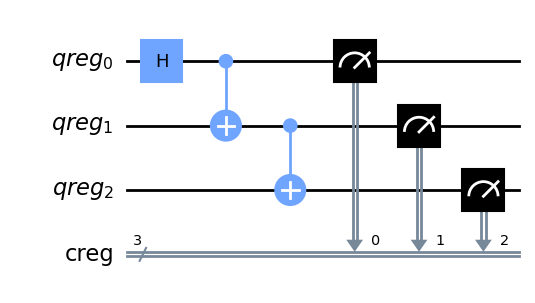
\includegraphics[width=\linewidth]{figs/GHZ.png}
    \caption{The circuit needed to initialize the GHZ state for three qubits.}
    \label{fig:GHZ_circ}
\end{figure}
Hadamard gates changes the basis of the gate between Pauli Z and Pauli X basis. CNOT changes the affected gate, based on the state of the control state. Visually, in a circuit, this can be presented as shown in Fig(\ref{fig:GHZ_circ}).
The result is a full entanglement, as seen in Fig(\ref{fig:qshpere}), where the outcome of any measurement on any qbit, will ascertain the outcome of all other measurements, as shown in Fig(\ref{fig:GHZ_measure}).
\begin{figure}[H]
    \centering
    \begin{subfigure}{0.48\textwidth}
        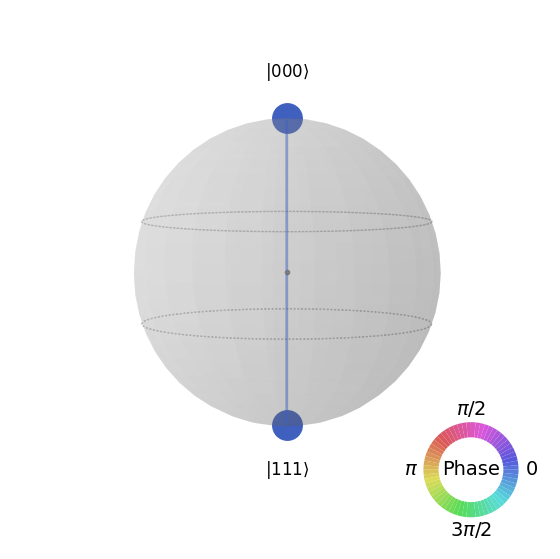
\includegraphics[width=\textwidth]{figs/GHZ qsphere.png}
        \caption{The Bloch-sphere representation of the GHZ state, given three qubits. It is strictly entangled, by their parallell nature.}
        \label{fig:qshpere}
    \end{subfigure}
    \hfill
    \begin{subfigure}{0.48\textwidth}
        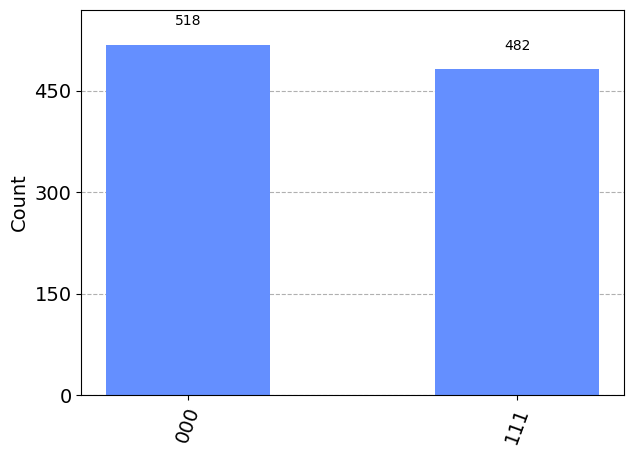
\includegraphics[width=\textwidth]{figs/GHZ Counts.png}
        \caption{The outcome of measurements of the GHZ state with three qubits.}
        \label{fig:GHZ_measure}
    \end{subfigure}
\end{figure}
Another important set of gates are the \textit{rotation operators} $R_x, R_y$ and $R_z$. By application to a qbit, we can reach any point on the Bloch sphere by usage of all three once. They are expressed as
\begin{align}
    \begin{split}
        R_x(\theta) &= \exp{-iX\theta/2} = \begin{pmatrix}
            \cos(\theta/2) & -i\sin(\theta/2) \\
            -i\sin(\theta/2) & \cos(\theta/2)
        \end{pmatrix}, \\
        R_y(\theta) &= \exp{-iY\theta/2} = \begin{pmatrix}
            \cos(\theta/2) & -\sin(\theta/2) \\
            -\sin(\theta/2) & \cos(\theta/2)
        \end{pmatrix}, \\
        R_z(\theta) &= \exp{-iZ\theta/2} = \begin{pmatrix}
            \exp{-i\theta/2} & 0 \\
            0 & \exp{i\theta/2}
        \end{pmatrix}
    \end{split}\label[eq]{eq:theo:bloch_rotations}
\end{align}
with all having a period of $4\pi$.

\subsection{Pauli Encoding Hamiltonians}
To apply a specific system to VQE, the Hamiltonian must be re-written in terms of a sum of \textit{Pauli strings}. Considering the identity $I$ and the three Pauli matrices $X, Y, Z$, we construct a specific term as a tensor product of these $P_i$. For an $n$-qubit system, we require $n-1$ tensor products. Combined with a weight $w_i$, the Hamiltonian must be written in the from
\begin{align}
    H = \sum_i w_i P_i \label[eq]{eq:theo:pauli_encoding_general}
\end{align}
For a general two-body Hamiltonian, this task can serve challenging. Many schemes exists for this purpose, such as the Jordan-Wigner transformation \citep{steudtnerMethodsSimulateFermions2019}. For the Lipkin model, an easier approach is available since the Hamiltonian can be written as products of the number and spin operators.


\subsection{Variational Quantum Eigensolver}
In this section we will briefly remind the reader of some key aspects of the variational method, followed by an outline on how observable values can be calculated using a QC. 

\subsubsection{Brief Remainder of the Variational Method}
The Rayleigh-Ritz VM states that for a given Hamiltonian $H$, the expectation value of a \textit{trial state} or \textit{ansatz} $\ket{A}$ puts a lower bound on the ground state energy $E_0$.
\begin{equation}
    \frac{\bra{A}H\ket{A}}{\ip{A}} \geq E_0
\end{equation}
The ansatz is typically chosen to be a parameterized superposition of basis states that can be varied to improve the energy estimate, $\ket{A}\equiv \ket{A(\boldsymbol{\theta})}$ where $\boldsymbol{\theta} = (\theta_1, \ldots, \theta_M)$ are the $M$ optimization parameters.

This is a crucial method in many-body theory, where good estimates of ground state energies are crucial due to the lack of analytical solutions. In contrast to perturbation theory, the VM will not give too small ground state energies, assuming that the ansatz has some overlap with the true ground state. The VM machinery form the basis of the VQE. 

\subsubsection{Algorithm}
We wish to apply the VM to estimate the ground state energy of a Hamiltonian on a quantum computer. To have any flexibility in the ansatz $\ket{A}$, we need to allow for parametrization. The most common approach is the so-called $RY$ ansatz, where we apply chained operations of rotating around the $y$-axis (\cref{eq:theo:bloch_rotations}) by $\boldsymbol{\theta} = (\theta_1,\ldots,\theta_Q)$ of the Bloch sphere and CNOT operations (\cref{eq:theo:CNOT_Hadamard}). Applications of $y$ rotations specifically ensures that our coefficients always remain real, which often is satisfactory when dealing with many-body systems. 
\newline
After the ansatz construction has been performed, the Hamiltonian must be applied. As discussed, the Hamiltonian must be written in terms of Pauli strings such that it is expressible as \cref{eq:theo:pauli_encoding_general}. To obtain the expectation value of the ground state energy, one can measure the expectation value of each Pauli string,

\begin{align*}
    E(\boldsymbol{\theta}) = \sum_i w_i\bra{A(\boldsymbol{\theta})} P_i \ket{A(\boldsymbol{\theta})} \equiv \sum_i w_i f_i,
\end{align*}
where $f_i$ is the expectation value of the Pauli string $i$. This is estimated statistically by considering measurements in the appropriate basis of the operator in the Pauli string. If the $P_i \supseteq Z_1$ we simply subtract the $0$ and $1$ outcomes of the first qbit, averaged over all measurements. If however we also have $P_i \supseteq X_2$, the second qbits measurement must be taken along the $x$-axis\footnote{To do this, we must must transform the qbit from the Pauli $z$-basis to the Pauli $x$-basis by application of a Hadamard gate.}. This with $N_0$ and $N_1$ as the number of $0$ and $1$ measurements respectively, we can estimate $f_i$ since 
\begin{align*}
    f_i = \lim_{N \to \infty} \frac{N_0 - N_1}{N},
\end{align*}
with $N$ as the number of shots (measurements). Therefor each Pauli string requires it own circuit, where multiple measurements of each string is required. Adding the results together with the corresponding weights, the ground state energy can be estimated. To optimize wrt. $\boldsymbol{\theta}$, a classical optimizer is often applied. Gradients are estimated using a simple finite difference approximation

\begin{align}
    \nabla_{\boldsymbol{\theta}} E(\boldsymbol{\theta}) \approx \frac{E(\boldsymbol{\theta} + \delta \boldsymbol{\theta})-E(\boldsymbol{\theta} - \delta \boldsymbol{\theta})}{2\delta \theta} ,
\end{align}
where $\delta \boldsymbol{\theta} = (\delta \theta, \ldots, \delta \theta)$. By updating the previous $\boldsymbol{\theta}$ values with some scalar times the negative of the gradient estimate, a new set of $\boldsymbol{\theta}$ values are obtained. The process is then repeated a finite amount of steps, where we hope to converge to the global minimum. A schematic of the procedure is presented in \cref{fig:VQE_scheme}. \newline An essential facet to this problem is the choice of an ansatz which will achieve a varied initial state, that can be altered through the optimization, furthering searches for better initial states. The ansatz used in this paper is shown in Fig(\ref{fig:ansatz}), and is taken from the article by Hlatshwayo et al. \cite{hlatshwayoSimulatingExcitedStates2022}

\begin{figure}[H]
    \centering
    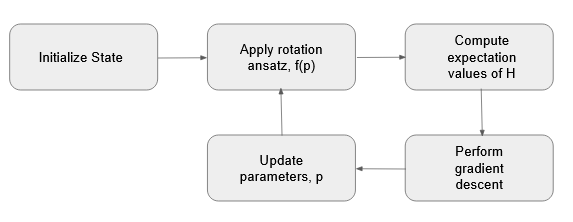
\includegraphics[width=\linewidth]{figs/VQE.PNG}
    \caption{A schematic of the process of Variational Quantum Eigensolvers.}
    \label[fig]{fig:VQE_scheme}
\end{figure}
\begin{figure}[H]
    \centering
    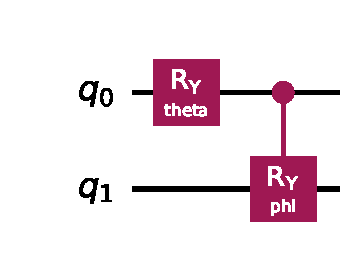
\includegraphics[width=\linewidth]{figs/ansatz.pdf}
    \caption{The ansatz for the VQE scheme applied for N = 4. }
    \label[fig]{fig:ansatz}
\end{figure}
